% TimeJEPA technical report.
% Build: make  (tectonic, or pdflatex+bibtex chain)
%
% House rules (do not violate when editing):
%   * no em-dashes anywhere
%   * every GIFT-Eval aggregate appears both plain and with flip TTA
%   * every claim points to its experiment; negative results stay in
%   * tell less, show more: prefer a table or figure over a paragraph
%   * grep PENDING to find spots awaiting running results
\documentclass[11pt,a4paper]{article}

\usepackage[T1]{fontenc}
\usepackage[utf8]{inputenc}
\usepackage{lmodern}
\usepackage{microtype}
\usepackage[margin=2.6cm]{geometry}
\usepackage{amsmath,amssymb}
\usepackage{booktabs}
\usepackage{graphicx}
\usepackage{xcolor}
\usepackage{tikz}
\usetikzlibrary{positioning,arrows.meta,fit,calc}
\usepackage{pgfplots}
\pgfplotsset{compat=1.17}
\usepackage[numbers,sort&compress]{natbib}
\usepackage[hidelinks]{hyperref}

\newcommand{\pending}[1]{\textcolor{gray}{[pending: #1]}}
% GIFT-Eval aggregate pair: MASE ratio / CRPS ratio vs seasonal naive
\newcommand{\gpair}[2]{#1\,/\,#2}

\title{TimeJEPA: What 1.1M Parameters\\and Joint Embeddings Can Do}
\author{Yvann Vincent\\
EFREI Paris\\
\texttt{yvann.vincent@gmail.com}}
\date{August 2026 \\ \small Working draft, updated as experiments complete.}

\begin{document}
\maketitle

\begin{abstract}
TimeJEPA is a 1.14M-parameter univariate forecaster pretrained with a
joint-embedding predictive architecture (JEPA) and evaluated zero-shot on
all 97 GIFT-Eval configurations with one checkpoint, one configuration, and
no adaptation of any kind. It reaches \gpair{0.863}{0.596} (MASE/CRPS
geometric-mean ratios vs seasonal naive, with sign-flip test-time
augmentation; \gpair{0.895}{0.624} without), between Moirai-large (311M) and
Moirai-base (91M) on the CRPS ranking, trained on three RTX~3090s. The
project's founding bet was that latent extrapolation is the right
pretraining objective for long-horizon forecasting. We pre-registered
predictions, ran the paired ablations, and the bet lost: the latent
objective is indistinguishable from reconstruction at equal budget, and its
apparent long-horizon advantage lives at rollout boundaries, not within the
window. Two things won instead. The corpus: every accuracy jump traces to
data composition, not to the objective. And the latent as a \emph{judge}:
the frozen pretrained energy ranks true futures far above chance, improves
TTM-R3 on five of six datasets as a zero-training reranker, and a
4-dimensional residual-statistics latent, gated into the quantile head,
carries the entire calibration of the forecast distribution (switching it
off costs 18.7 CRPS points; the median is invariant by construction). The
corpus makes the forecast; the latent makes the judge. All numbers trace to
a dated, pre-registered experimental log.
\end{abstract}

\section{Introduction}
\label{sec:intro}

This paper reports a model and the fate of the idea behind it. Both matter.

The idea: in I-JEPA \citep{assran2023ijepa} the predictor is scaffolding,
discarded after pretraining. TimeJEPA inverts that. The predictor
extrapolates the future in latent space and is kept as the inference organ;
the decoder is a reading head. The bet, registered before any measurement:
latent extrapolation is the right pretraining task for a forecaster.
Forecasting is generation, not infilling, the causal/masked split of
language modeling \citep{radford2018gpt,devlin2019bert}; the irreducibly
unpredictable share of a series' future is enormous, and a latent loss lets
the EMA target encoder absorb it \citep{lecun2022path}; transfer should be
clean.

We tested the bet the way we tested everything: paired runs, one variable
each, numeric predictions written into a dated log before results. The bet
lost. At equal corpus and budget, latent extrapolation and reconstruction
differ by 1.4\%, and reconstruction wins most paired cells
(Section~\ref{sec:objective}). A monotone long-horizon advantage did appear
on GIFT-Eval (+0.8/+3.1/+6.6\% over short/medium/long), then a per-step
analysis killed the obvious reading: within a window the advantage
\emph{shrinks} with depth (slope $-1.64\%$ per 100 steps, CI excluding
zero). What survives is narrower and unconfirmed: the latent objective may
degrade less under iteration on its own outputs.

What moved the numbers instead was data. The full trajectory from
\gpair{0.979}{0.677} to \gpair{0.863}{0.596} (Figure~\ref{fig:progression})
decomposes into protocol, geometry, corpus, normalization, synthetic data,
batch rationing, checkpoint selection, and one test-time symmetry. The
pretraining objective contributed nothing measurable. The field is currently
excited about JEPA for time series; our evidence says that as a way to make
a small model forecast better, it is not where the leverage is.

The latent earns its keep elsewhere. A pretrained JEPA is implicitly an
energy over (context, future) pairs, and that energy is a competent
\emph{judge}: it ranks true futures far above chance, improves TTM-R3 on
five of six datasets as a frozen zero-training reranker, and a
4-dimensional latent trained to predict residual statistics carries the
entire calibration of the quantile fan, an 18.7-point CRPS ablation with
the median invariant by construction (Section~\ref{sec:judge}). One
sentence summarizes twenty experiments: \emph{the corpus makes the
forecast; the latent makes the judge.}

Three evaluation properties frame every number. One checkpoint and one
configuration serve all 97 GIFT-Eval configurations; no per-regime variants
(the TTM family publishes several). Nothing is tuned, calibrated or
selected on GIFT-Eval data. The compute budget is three RTX~3090s; every
experiment here is re-runnable by one person on one machine.

\section{Related work}
\label{sec:related}

\paragraph{Time series foundation models.}
No paradigm has swept the field: decoder-only (TimesFM
\citep{das2024timesfm}, Toto \citep{cohen2024toto}), masked encoder (Moirai
\citep{woo2024moirai}, whose LOTSA corpus we pretrain on), tokenized
seq-to-seq (Chronos \citep{ansari2024chronos}), xLSTM (TiRex
\citep{auer2025tirex}), state space (FlowState \citep{flowstate2025}), MLP
mixers (TTM \citep{ekambaram2024ttm}) all compete on GIFT-Eval
\citep{aksu2024gifteval}. Size is not the lever: Toto spans 4M to 1B
parameters, a factor of 250, for 4.6 CRPS points, and sub-10M models
(TTM-R3, FlowState, TinyCast) beat much larger ones. That is TimeJEPA's
class, and why testing \emph{which pretraining objective} serves
forecasting at fixed small capacity has a place. Other reference points:
Lag-Llama \citep{rasul2023lagllama}, Timer \citep{liu2024timer}, Sundial
\citep{liu2025sundial}, VisionTS \citep{chen2024visionts}, YingLong
\citep{yinglong2025}, DeepAR \citep{salinas2020deepar}, TiDE
\citep{das2023tide}.

\paragraph{JEPA and self-supervised learning.}
JEPA was proposed as a path to predictive world models \citep{lecun2022path}
and instantiated for images and video
\citep{assran2023ijepa,bardes2024vjepa,assran2025vjepa2}, always with a
disposable predictor. Anti-collapse machinery: BYOL's EMA target
\citep{grill2020byol} with the MoCo~v3 momentum schedule
\citep{chen2021mocov3}, VICReg \citep{bardes2022vicreg}, and LeJEPA's SIGReg
\citep{balestriero2025lejepa}, our default. Our energy reading of the
latent follows \citet{lecun2006ebm}. To our knowledge TimeJEPA is the first
systematic attempt to keep the JEPA predictor as the forecasting organ for
time series and measure whether that helps.

\paragraph{Components, data, inference.}
Patching and channel independence follow PatchTST \citep{nie2023patchtst};
instance normalization follows RevIN \citep{kim2022revin}, composed with a
robust arcsinh transform whose precedent is Toto's scaler
\citep{cohen2024toto}; pre-norm blocks \citep{xiong2020preln} with rotary
embeddings \citep{su2024rope}. Quantile decoding optimizes pinball loss
\citep{koenker1978quantile,gneiting2007scoring}; metrics follow
\citet{hyndman2006mase} and GluonTS \citep{alexandrov2020gluonts}.
Synthetic pretraining data follows KernelSynth \citep{ansari2024chronos}
via random Fourier features \citep{rahimi2007rff}; CauKer adds causal
structure \citep{cauker2025}; Toto-2 reports a majority-synthetic recipe
\citep{khwaja2026toto2}; our shape augmentations follow the TiRex ablation
\citep{auer2025tirex}. Sign-flip test-time augmentation has precedents in
TimesFM and YingLong \citep{das2024timesfm,yinglong2025}; conformal
calibration follows \citet{romano2019cqr,vovk2005conformal}; weight
averaging \citep{izmailov2018swa,wortsman2022soups} failed cleanly for us.
The world-model perspective connects to
\citep{ha2018worldmodels,hansen2024tdmpc2,zhou2024dinowm,williams2017mppi};
our measured constraint, prudence from predicted uncertainty rather than
from the energy, converges with \citet{henaff2019mpur}.

\section{TimeJEPA}
\label{sec:architecture}

Figure~\ref{fig:arch} shows the model with its tensor shapes,
Table~\ref{tab:params} its measured parameter budget. Horizons beyond
the native 256 use a rollout that propagates the full quantile fan under
a comonotone coupling (Appendix~\ref{app:training}). Four design choices
were forced by measurements; everything else, each detail with its own
measurement, is in Appendix~\ref{app:training}.

\begin{figure*}[t]
\centering
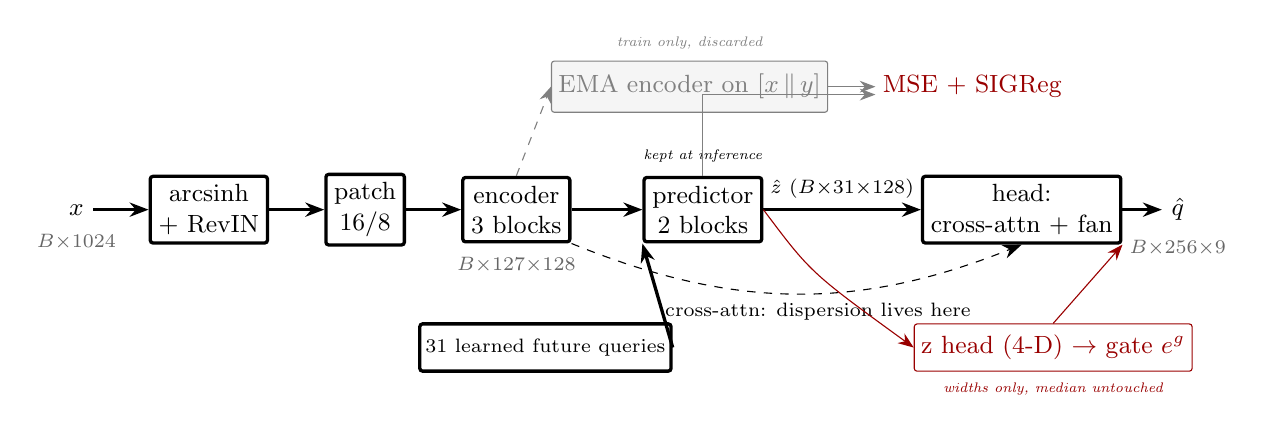
\begin{tikzpicture}[
  font=\small,
  box/.style={draw, very thick, rounded corners=1pt, minimum height=7.5mm, inner sep=3pt, align=center},
  gbox/.style={draw, gray, fill=gray!8, rounded corners=1pt, minimum height=6.5mm, inner sep=2.5pt, align=center, text=gray},
  zbox/.style={draw, red!60!black, rounded corners=1pt, minimum height=6mm, inner sep=2.5pt, align=center, text=red!60!black},
  shp/.style={font=\scriptsize, text=black!60, below=0.5mm},
  tag/.style={font=\tiny\itshape, above=0.2mm},
  arr/.style={-{Stealth[length=2.4mm]}, very thick},
  garr/.style={-{Stealth[length=2mm]}, gray},
  node distance=4mm and 7mm]
% inference line
\node (x) {$x$};
\node[shp, below=0mm of x] {$B{\times}1024$};
\node[box, right=of x] (norm) {arcsinh\\+ RevIN};
\node[box, right=of norm] (patch) {patch\\16/8};
\node[box, right=of patch] (enc) {encoder\\3 blocks};
\node[shp, below=0.5mm of enc] {$B{\times}127{\times}128$};
\node[box, right=9mm of enc] (pred) {predictor\\2 blocks};
\node[tag, above=0.5mm of pred] {kept at inference};
\node[box, right=20mm of pred] (qh) {head:\\cross-attn + fan};
\node (out) [right=5mm of qh] {$\hat q$};
\node[shp, below=0mm of out] {$B{\times}256{\times}9$};
% future queries
\node[box, below=10mm of pred, xshift=-20mm, minimum height=6mm, inner sep=2pt, font=\scriptsize] (fq)
  {31 learned future queries};
% pretrain branch
\node[gbox, above=8mm of enc, xshift=22mm] (tgt) {EMA encoder on $[x \,\Vert\, y]$};
\node[tag, above=0.2mm of tgt] {\color{gray}train only, discarded};
\node[gbox, right=6mm of tgt, draw=none, fill=none, text=red!60!black, font=\small] (jl)
  {MSE + SIGReg};
% z gate
\node[zbox, below=10mm of qh, xshift=4mm] (z) {z head (4-D) $\to$ gate $e^{g}$};
\node[tag, below=0.2mm of z, text=red!60!black] {widths only, median untouched};
\draw[arr] (x) -- (norm);
\draw[arr] (norm) -- (patch);
\draw[arr] (patch) -- (enc);
\draw[arr] (enc) -- (pred);
\draw[arr] (pred) -- node[above]{\scriptsize $\hat z$ ($B{\times}31{\times}128$)} (qh);
\draw[arr] (qh) -- (out);
\draw[arr] (fq.east) -- (pred.south west);
\draw[garr] (pred.north) |- ($(jl.west)+(0,-1mm)$);
\draw[garr] (tgt) -- (jl);
\draw[garr, dashed] (enc.north) -- (tgt.west);
\draw[arr, dashed, thin] (enc.south east) to[bend right=22]
  node[below, pos=0.55]{\scriptsize cross-attn: dispersion lives here} (qh.south);
\draw[-{Stealth[length=2mm]}, red!60!black] (pred.east) ..controls +(6mm,-8mm).. (z.west);
\draw[-{Stealth[length=2mm]}, red!60!black] (z.north) -- (qh.south east);
\end{tikzpicture}
\caption{TimeJEPA with tensor shapes. Bold: the inference path, all of
it kept, the predictor included (in I-JEPA it is scaffolding; here it is
the forecasting organ), with the future represented by 31 learned
queries, not teacher forcing. Gray: the pretraining branch, discarded at
inference. Dispersion is produced by the head's cross-attention to the
context, not by $\hat z$; the red gate multiplies fan widths only,
leaving the median untouched (Proposition~\ref{prop:median}).}
\label{fig:arch}
\end{figure*}

\begin{itemize}
\item \textbf{Geometry randomization at fine-tuning time.} Skill
initially peaked at the training context length and collapsed on both
sides ($+28.5\%$ skill at context 384, $-103.8\%$ at 768 on one
dataset): the model memorizes a patch count. Randomizing context and
horizon per batch flattens the sweep from 33\% spread to 5\%; a scratch
control attributes the robustness to fine-tuning-time randomization, not
pretraining.
\item \textbf{Robust normalization with a bounded inverse.} Inputs pass
through $N(x) = \operatorname{arcsinh}((x - \mathrm{med}(c))/s(c))$ with
a robust floored scale $s$, then RevIN \citep{kim2022revin}; the inverse
clamps to a context envelope (precedents: Toto's scaler
\citep{cohen2024toto}, Chronos's $\pm 15\sigma$ vocabulary
\citep{ansari2024chronos}). What test-time symmetries survive this
normalization is settled below.
\item \textbf{A quantile head that attends back to the context.} The
MSE-trained predictor converges toward a conditional mean (measured:
predicted-latent variance 0.6 vs target 0.95), so dispersion cannot live
in $\hat z$; the head cross-attends to context embeddings and decodes
\begin{equation}
\hat q_{\tau_j} = \hat q_{0.5} \pm \textstyle\sum_{i \le j}
\operatorname{softplus}(w_i),
\label{eq:fan}
\end{equation}
a fan that cannot cross by construction. Direct quantiles optimize the
benchmark metric with no proxy; the median is the MASE-optimal point
\citep{koenker1978quantile,hyndman2006mase}.
\item \textbf{A zero-initialized gate for residual statistics.} A 4-D
head on the predictor trunk multiplies the widths of
Eq.~\ref{eq:fan} by $e^{g}$, zero-initialized: exact identity at the
start of fine-tuning, with consequences made precise below
(Section~\ref{sec:esjepa}).
\end{itemize}

\begin{table}[b]
\centering
\small
\begin{tabular}{lrr}
\toprule
Component & Params & Share \\
\midrule
Patch embedding & 2{,}432 & 0.2\% \\
Online encoder & 595{,}072 & 52.4\% \\
Predictor & 419{,}968 & 37.0\% \\
Quantile head & 118{,}162 & 10.4\% \\
RevIN affine & 2 & \\
\midrule
Trainable total & \textbf{1{,}135{,}636} & \\
EMA target copy (frozen) & 595{,}072 & \\
\bottomrule
\end{tabular}
\caption{Measured parameter decomposition.}
\label{tab:params}
\end{table}


\begin{lemma}[affine quotient]
\label{lem:affine}
Let $N(x) = \operatorname{arcsinh}((x - \mathrm{med}(c))/s(c))$ with
$s$ 1-homogeneous (ours, away from its numerical floor). For every
$k > 0$ and $b$, $N(kx + b) = N(x)$: the normalization quotients the
positive affine group. For the reflection, $N(-x) = -N(x)$.
\end{lemma}
\begin{proof}
$\mathrm{med}(kx{+}b) = k\,\mathrm{med}(x){+}b$ and
$s(kx{+}b) = k\,s(x)$, so the argument of $\operatorname{arcsinh}$ is
unchanged; under $x \mapsto -x$ it changes sign, and
$\operatorname{arcsinh}$ is odd.
\end{proof}

Two consequences, both used: test-time scale augmentation is the
identity (Table~\ref{tab:tta}, pinned by a bit-identity test), and the
sign is the only affine symmetry left, which yields the flip formula of
Section~\ref{sec:results}.

\begin{proposition}[median invariance]
\label{prop:median}
In Eq.~\ref{eq:fan} with gated widths
$\operatorname{softplus}(w_i)\,e^{g}$, the median $\hat q_{0.5}$ does
not depend on $g$. At fixed weights, any change in CRPS or coverage
under gate surgery is therefore attributable to the spread, and MASE is
structurally invariant.
\end{proposition}
\begin{proof}
By inspection: $g$ enters only the summed width terms.
\end{proof}

Pretraining is standard JEPA: MSE to EMA-encoded targets plus SIGReg
\citep{balestriero2025lejepa} (a VICReg control was indistinguishable),
AdamW at $3\times10^{-4}$ cosine, bf16, batch 512 per GPU
(Appendix~\ref{app:training}).

\section{Pretraining, and the fate of the founding hypothesis}
\label{sec:objective}

\paragraph{Objective.}
Standard JEPA plus one term:
\begin{equation}
\mathcal{L} = \operatorname{MSE}(\hat z, z_{\mathrm{tgt}})
+ \lambda\,\Omega(z_{\mathrm{ctx}})
\;[+\; \lambda_z \operatorname{SmoothL1}(\hat s, s)],
\end{equation}
with $\Omega$ = SIGReg \citep{balestriero2025lejepa} at $\lambda{=}1$ (16
random 1-D projections pushed toward Gaussian; VICReg control was
indistinguishable, 1.193 vs 1.183 average MASE, but SIGReg constrains the
whole distribution where a variance hinge accepts bimodal collapse). The
bracketed term is the ESJEPA arm ($\lambda_z{=}0.1$,
Section~\ref{sec:esjepa}). Two implementation lessons that cost real
results: compute variance statistics per patch position, not pooled
(pooled 0.9990 vs per-position 0.0000, positional diversity masking true
collapse), and never regularize a detached tensor (zero gradient, inflated
reported loss). AdamW \citep{loshchilov2019adamw}, peak LR
$3\times10^{-4}$, warmup 10\% then cosine, bf16, batch 512 per GPU on three
3090s. The LR ceiling and the short budgets are measurements, not habits: a
cosine calibrated for 40 epochs never decays in 3 (the run oscillated,
0.345--0.445, and its ``best checkpoint'' was a noise trough), and the full
corpus is exhausted in about one epoch, after which validation rises.
Collapse is monitored by per-position std and effective rank, calibrated
per corpus (rank at init: 3.7--4.8 on Monash, 43--87 on LOTSA).

\subsection{The founding bet, tested to destruction}
\label{sec:hypothesis}

The claim under test: latent extrapolation beats reconstruction as a
pretraining objective, increasingly so at long horizon. Four measurements,
in order.

\textbf{1. The paired duel is null.} One-variable reconstruction arm
(decode to normalized patches, SmoothL1, no anti-collapse: fixed targets
cannot collapse), checkpoints paired at 0.4\% val loss. Seven-dataset MASE:
latent 1.150, reconstruction 1.166. Reconstruction wins 17/28 paired cells,
median gap 0.5\% in its favor. GIFT-Eval: \gpair{0.979}{0.6766} vs
\gpair{1.003}{0.6764}, identical CRPS. Verdict: not ``JEPA loses'' but
``indistinguishable,'' which suffices to strike the claim.

\textbf{2. A horizon signal appeared and replicated.} Latent advantage
monotone in the GIFT term: $+0.8\%$ (short, $n{=}55$), $+3.1\%$ (medium,
$n{=}21$), $+6.6\%$ (long, $n{=}21$); same pattern in the Nixtla cells.
For a week this was the thesis.

\textbf{3. The per-step analysis killed the obvious mechanism.} If
predicting far is cheaper in latent space, the gap must grow with depth
\emph{inside} a window. Paired bootstrap over per-step MAE, eight datasets,
20{,}000 resamples: the gap \emph{shrinks} with depth, slope $-1.64\%$ per
100 steps, 95\% CI $[-2.82, -0.56]$, negative in 6/8 datasets. Across
rollout counts the picture inverts: gap vs number of rolls, Spearman
$+0.404$, $p{=}0.019$; latent significantly \emph{worse} at h192
(single window), ahead only at h720 (three rolls). Surviving candidate:
\emph{the latent objective degrades less under iteration on its own
outputs}. Fragile ($p{=}0.069$ without one dataset), with a registered
three-seed protocol not yet funded. A native h512 fine-tune (grown query
table, same pretrain, halving the roll count for the affected horizons)
supplied a paired check: on configurations unaffected by a window-induced
corpus change (Section~\ref{sec:results}), the multi-rollout group improved
by 1.7\% relative to the single-roll group, the sign the boundary
hypothesis predicts and the magnitude of a minor lever, consistent with the
flat term aggregates.

\textbf{4. What pretraining itself buys.} Against from-scratch at equal
fine-tuning: in-domain, nothing (1.193 vs 1.187, strict equality); on
never-fine-tuned datasets, $-26\%$ MASE on 8/8 (upper bound: the strongest
dataset was later found contaminated, Appendix~\ref{app:pitfalls}), tightened
to $-8.7\%$ in a budget-controlled clean rerun. Pretraining does not
improve fit; it improves transfer. And note the selector trap: fine-tuning
validation loss preferred the wrong model (0.159 scratch vs 0.181
pretrained) while the pretrained one transferred better.

One argument for JEPA survives untouched, and it is architectural, not
empirical: latents allow equivariance by objective. A context at
resolution $k_1$ and a target at $k_2$ can be tied through a predictor
conditioned on $w{=}k_2/k_1$; reconstruction cannot do this, two
resolutions do not share target values. Built (the FiLM path), never
funded. It is the cleanest reason to keep the formulation.

\section{Corpus}
\label{sec:corpus}

Real data is LOTSA \citep{woo2024moirai}, split into univariate
channels, with every subset matching an evaluation benchmark excluded by
verified name patterns (all 28 GIFT-Eval datasets plus the Nixtla suite,
whole datasets, pinned by a non-regression test); our patterns are
strictly stricter than Salesforce's own sanctioned pretraining corpus at
a quantified cost of 0.9\% of observations
(Appendix~\ref{app:corpus}).

Batches are drawn with square-root temperature weighting and a $3\times$
oversampling cap, \emph{rationed}: consumed greedily, the cap makes
small families vanish early and batch composition drift through the
epoch; converting it to a fractional per-batch quota makes composition
stationary, and the rationed run produced the CRPS champion
(Appendix~\ref{app:corpus}).

54\% of the served batch is synthetic, a dose that is audited rather
than estimated. It exists because the per-configuration error map showed
holes exactly where no real data can be added: a frequency gap between
5-minute and hourly sampling, short yearly shapes rejected by chunking,
and two morphologies with no public data at all, bursty IT-operations
series and intermittent integer counts, generated by a
random-Fourier-feature KernelSynth
\citep{ansari2024chronos,rahimi2007rff} plus dedicated samplers.
Shape augmentations follow the TiRex ablation \citep{auer2025tirex};
scale augmentation is inert under the normalization
(Lemma~\ref{lem:affine}), so the budget goes entirely to shape.

\section{Evaluation protocol}
\label{sec:protocol}

One checkpoint and one configuration serve all 97 GIFT-Eval
configurations: same weights, same context, same decoding, horizons beyond
256 by the model's own rollout, and nothing anywhere tuned or selected on
GIFT-Eval data. The harness restates the official protocol next to its
upstream sources rather than importing it; convention drift against the
official CSVs is measured and printed (zero on MASE, about 2.7\% on
CRPS). Missing targets are masked, never imputed; aggregates are
geometric means of per-configuration ratios against seasonal naive. A full
97-configuration pass takes about four minutes on one GPU, which is what
makes checkpoint selection by evaluation affordable: fine-tuning
validation loss reliably designates the wrong checkpoint, even when the
validation curve is clean (Section~\ref{sec:negative}).

The single test-time augmentation is the sign flip,
\begin{equation}
\hat{q}_\tau(x) = \tfrac{1}{2}\left[\, q_\tau(x) - q_{1-\tau}(-x) \right],
\label{eq:flip}
\end{equation}
correct for a distributional forecast since $q_\tau(-X) = -q_{1-\tau}(X)$,
with precedents in TimesFM and YingLong
\citep{das2024timesfm,yinglong2025}; it buys $-2.0\%$ MASE and $-2.4\%$
CRPS at $2\times$ forward cost. Table~\ref{tab:tta} shows why flip is
alone: under a normalization that quotients the affine group, the sign is
the only symmetry left, and the measured alternatives are null or
negative. Every aggregate in this paper appears both plain and with flip,
and we refuse multi-checkpoint ensembling.

\begin{table}[t]
\centering
\small
\begin{tabular}{llll}
\toprule
Variant & MASE & CRPS & Verdict \\
\midrule
none (champion, plain) & 0.895 & 0.624 & reference \\
sign flip (Eq.~\ref{eq:flip}) & \textbf{0.870} & \textbf{0.596} & official ($2\times$ cost) \\
scale $f(kx)/k$ & = & = & provable no-op (pinned by test) \\
translation (shifts 1--7) & 0.898 & 0.627 & negative: staleness beats phase \\
multi-lookback \{512,1024\} & 0.896 & 0.623 & mixed alone, worse with flip \\
context 2048 at inference & 1.190 & 0.876 & collapse; long context must be trained \\
\bottomrule
\end{tabular}
\caption{Test-time variants on the rationed champion.}
\label{tab:tta}
\end{table}

\section{Protocol and results}
\label{sec:results}

\paragraph{Protocol.}
One checkpoint, one configuration, all 97 configurations; nothing tuned
or selected on GIFT-Eval data. The harness restates the official
protocol next to its sources (measured convention drift: zero on MASE,
$\sim$2.7\% on CRPS); aggregates are geometric-mean ratios vs seasonal
naive. Checkpoints are selected by intermediate evaluation, a doctrine
forced by measurement: validation loss designated the wrong checkpoint
three times out of three, once with a perfectly clean curve. The single
test-time augmentation is the sign flip,
$\hat{q}_\tau(x) = \tfrac{1}{2}[q_\tau(x) - q_{1-\tau}(-x)]$, the one
symmetry Lemma~\ref{lem:affine} leaves; precedents include TimesFM,
YingLong, and the 0.15M TinyCast
\citep{das2024timesfm,yinglong2025}. Table~\ref{tab:tta} shows why it
is alone. We refuse multi-checkpoint ensembling, and report every aggregate
plain and with flip.

\begin{table}[t]
\centering
\scriptsize
\begin{tabular}{llll}
\toprule
Variant & MASE & CRPS & Verdict \\
\midrule
none (champion, plain) & 0.895 & 0.624 & reference \\
sign flip & \textbf{0.870} & \textbf{0.596} & official ($2\times$ cost) \\
scale $f(kx)/k$ & = & = & identity (Lemma~\ref{lem:affine}) \\
time shift (origins $-1..{-7}$) & 0.898 & 0.627 & staleness beats phase \\
multi-lookback & 0.896 & 0.623 & worse with flip \\
context 2048 at inference & 1.190 & 0.876 & must be trained \\
\bottomrule
\end{tabular}
\caption{Test-time variants: under a normalization that quotients the
affine group, the sign is the only symmetry left.}
\label{tab:tta}
\end{table}

\begin{figure*}[t]
\centering
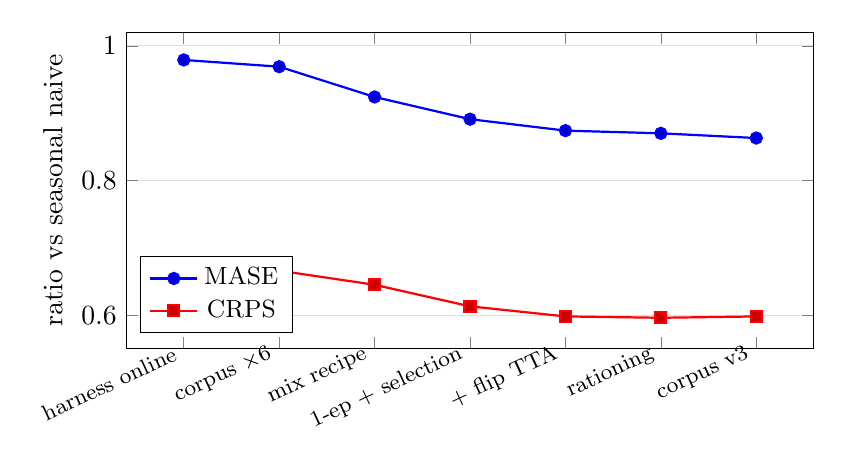
\begin{tikzpicture}
\begin{axis}[
  width=0.85\textwidth, height=5.6cm,
  ymin=0.55, ymax=1.02,
  ylabel={ratio vs seasonal naive},
  symbolic x coords={harness online, corpus $\times$6, mix recipe, 1-ep + selection, + flip TTA, rationing, corpus v3},
  xtick=data, x tick label style={rotate=25, anchor=east, font=\footnotesize},
  ymajorgrids, grid style={gray!25},
  legend style={font=\small, at={(0.02,0.05)}, anchor=south west},
  every axis plot/.append style={thick, mark=*}]
\addplot coordinates {(harness online,0.979) (corpus $\times$6,0.969)
  (mix recipe,0.924) (1-ep + selection,0.891) (+ flip TTA,0.874)
  (rationing,0.870) (corpus v3,0.863)};
\addplot coordinates {(harness online,0.677) (corpus $\times$6,0.666)
  (mix recipe,0.645) (1-ep + selection,0.613) (+ flip TTA,0.598)
  (rationing,0.596) (corpus v3,0.598)};
\legend{MASE, CRPS}
\end{axis}
\end{tikzpicture}
\caption{GIFT-Eval aggregates across the project, each step labeled by
the single change responsible. Every step is a data or inference change;
the objective contributes none, and volume alone is the weakest lever
(corpus $\times 6$ buys 1.6\% CRPS). The last three CRPS points agree to
$\pm 0.002$.}
\label{fig:progression}
\end{figure*}

\begin{table}[t]
\centering
\scriptsize
\begin{tabular}{lrccl}
\toprule
Model & Params (M) & CRPS & MASE & Notes \\
\midrule
TinyCast & 0.1 & 0.545 & 0.774 & \\
TTM-R3 & 1.4 & 0.520 & 0.724 & per-regime configs \\
\textbf{TimeJEPA} & \textbf{1.1} & \textbf{0.596} & \textbf{0.863} & one config, flip \\
Lag-Llama & 2.4 & 0.880 & 1.228 & leakage flagged \\
Toto-2.0-4m & 4.1 & 0.524 & 0.757 & \\
YingLong-6m & 7.3 & 0.609 & 0.880 & \\
FlowState & 9.1 & 0.502 & 0.726 & \\
Kairos-10m & 9.9 & 0.554 & 0.753 & \\
Moirai2 & 11.4 & 0.516 & 0.728 & \\
\midrule
Moirai-large & 311.0 & 0.599 & & adjacent rank \\
TimesFM-2.5 & 231.3 & 0.490 & & \\
Chronos-2 & 119.5 & 0.485 & & \\
Seasonal naive & & 1.000 & 1.000 & \\
\bottomrule
\end{tabular}
\caption{The sub-12M class on GIFT-Eval (frozen snapshot; metadata is
the leaderboard's own). TimeJEPA ranks $\sim$91st of 125 on CRPS,
between FLAIR and Migas-1.0, ahead of Moirai-large, and seventh of the
eight zero-shot sub-12M entries shown: mid-board overall, lower-third
in its class, and the only entry trained on three consumer GPUs. The
paper's claims do not rest on this rank.}
\label{tab:small-models}
\end{table}

\paragraph{Where the remaining gap lives.}
Two floors. The \emph{tail}: sixteen configurations above ratio 1.25
cost about 12 aggregate points before the synthetic recipe compressed
them to six, exactly as pre-registered; the residual tail is what the
newest synthetic families target. The \emph{body}: on the other 81
configurations we sit near 0.54 where the sub-10M leaders sit near
0.47, diffuse, no single culprit; term aggregates are flat, so the
rollout is not the bottleneck.

\paragraph{A recipe ceiling, not a capacity ceiling.}
Three fine-tunes from three pretrains on three corpus recipes land at
flip CRPS $0.597 \pm 0.002$: our levers are exhausted at this size. The
cross-sectional evidence rules out raw capacity as the binding
constraint (TinyCast reaches 0.545 with 0.15M parameters, FlowState-3M
0.496 \citep{flowstate2025}), and names the candidate walls: both
sub-3M leaders train at long context (2048--4096) and treat time scale
explicitly, and FlowState's own three-seed ablation prices those levers
at $+0.051$ CRPS (sampling-rate equivariance) and $+0.046$ (parallel
multi-horizon forecasts), together approximately our entire 0.094 gap.
A $\times 3$ model under the identical recipe, bands registered in
advance, is in progress to measure the capacity share of the ceiling;
the equivariance lever is the unfunded cross-resolution arm of
Section~\ref{sec:objective}.
% PENDING(mini): the 3.4M model against its registered bands.
% PENDING(v3-final): plain pair of the v3 champion; late-checkpoint verdicts.

\section{The latent as judge}
\label{sec:judge}

A pretrained JEPA is implicitly an energy over (context, future) pairs,
$E(x, y) = 1 - \cos(\hat{z}(x), \mathrm{enc}([x \,\Vert\, y]))$
\citep{lecun2006ebm}, lowered on true pairs by the invariance term.
Everything below reads it off \emph{frozen} checkpoints.

\begin{figure*}[!t]
\centering
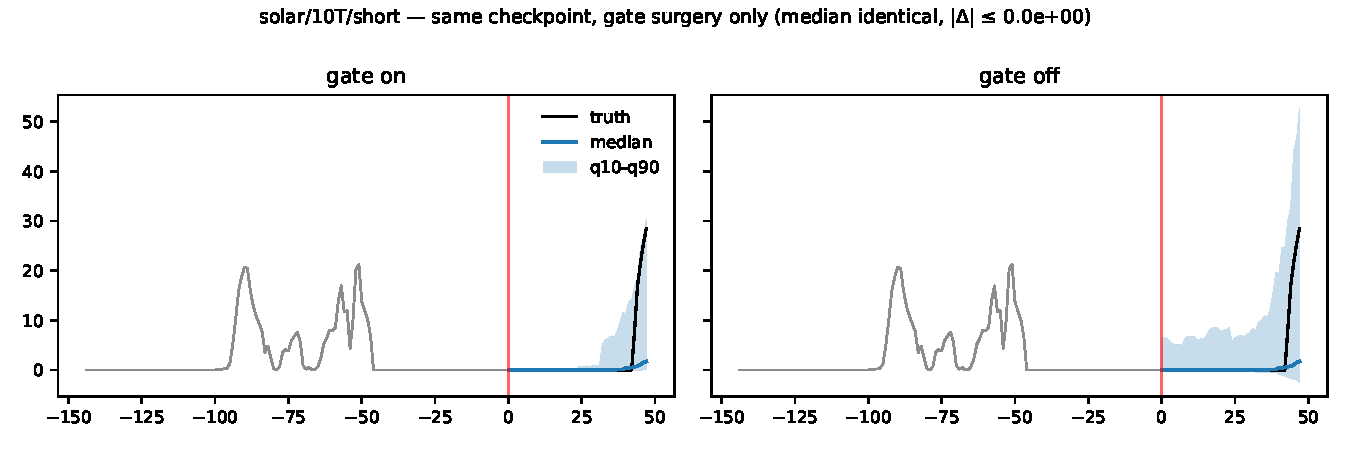
\includegraphics[width=0.92\textwidth]{figures/gate_fan_solar_10T_short.pdf}
\caption{The gate on one solar window (10-minute data), same checkpoint,
same median (max difference $0$), gate surgery only. With the gate, the
fan is pinned to zero through the night, where the outcome is certain,
and opens at sunrise; without it, the same weights spread a worst-case
envelope over certain zeros. Note that the truth briefly escaping the
band at the peak is what a calibrated 80\% interval is supposed to do
one step in five; the gate-off panel that covers everything is the 0.968
coverage pathology of Table~\ref{tab:esjepa} in picture form.}
\label{fig:gatefan}
\end{figure*}


\paragraph{The judge exists; fine-tuning destroys it.}
Figure~\ref{fig:probe}: pretrained checkpoints rank the true future at
0.21--0.25 among 34 candidates (chance 0.50; median rank 0.000 on hourly
electricity for the best judge), while a fully fine-tuned checkpoint
degrades to 0.41. The judge peaks early in pretraining and erodes while validation keeps
improving, so judge selection uses an early probe; it also scales with
capacity faster than forecasting does.

\begin{figure}[t]
\centering
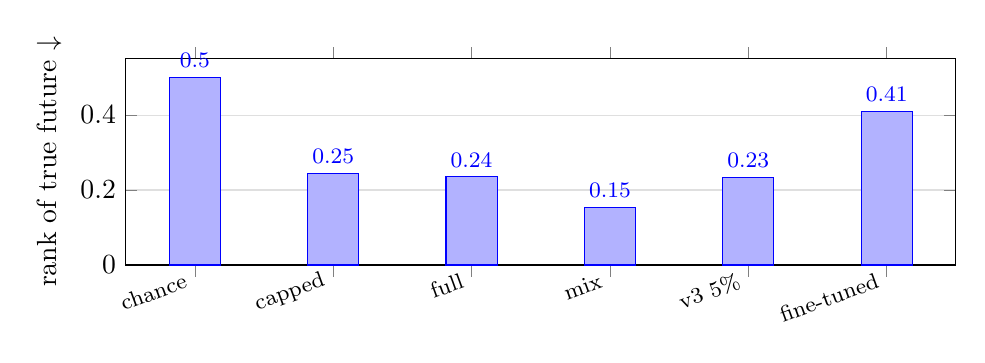
\begin{tikzpicture}
\begin{axis}[
  width=\columnwidth, height=4.2cm, ybar,
  ymin=0, ymax=0.55,
  ylabel={rank of true future $\downarrow$},
  symbolic x coords={chance, capped, full, mix, v3 5\%, fine-tuned},
  xtick=data, x tick label style={rotate=20, anchor=east, font=\footnotesize},
  bar width=6.5mm, ymajorgrids, grid style={gray!25},
  nodes near coords, every node near coord/.append style={font=\footnotesize}]
\addplot coordinates {(chance,0.50) (capped,0.245) (full,0.235)
  (mix,0.153) (v3 5\%,0.233) (fine-tuned,0.409)};
\end{axis}
\end{tikzpicture}
\caption{The judge lives in the pretrain and dies in the fine-tune
(normalized rank of the truth among 34 candidates; 0.50 is chance).}
\label{fig:probe}
\end{figure}

\paragraph{A zero-training reranker that upgrades TTM-R3
(Table~\ref{tab:hybrid}).}
Candidate futures are scored with $E$ and read out as weighted
quantiles; candidates share the proposer's center, and degenerate pools
fall back to uniform weights (pool design, and the four-fold dilution
replication that forced it, in Appendix~\ref{app:training}).

\begin{table}[t]
\centering
\scriptsize
\begin{tabular}{lcccccc}
\toprule
WQL vs SN $\downarrow$ & ettm1 & ettm2 & etth1 & etth2 & weather & exch. \\
\midrule
TTM-R3 alone & 0.88 & 0.81 & 0.85 & 0.95 & \textbf{0.63} & 0.88 \\
+ judge (centered) & \textbf{0.77} & \textbf{0.72} & \textbf{0.71} & \textbf{0.78} & 0.64 & \textbf{0.78} \\
\bottomrule
\end{tabular}
\caption{A frozen 1M judge turns a point forecaster into a probabilistic
one that beats or ties its own WQL on 6/6 held-out datasets, zero
additional training, replicated across judges from two pretraining
lineages. On all 97 GIFT configurations (paired windows) the pipeline
beats TTM's collapsed point CRPS by 7\% at a 3.8\% MASE tax; coverage
(0.62 vs 0.80 nominal) is the open gap. Given a deliberately biased
proposer, the judge moves its mass to the alternative center it keeps in
the pool: a verifier that can fire its proposer.}
\label{tab:hybrid}
\end{table}

\paragraph{Four dimensions carry the calibration
(Table~\ref{tab:esjepa}).}
\label{sec:esjepa}
The predictor converges to a conditional mean
(Section~\ref{sec:architecture}); rather than the residual, irrecoverable
by definition, a 4-D head predicts its \emph{statistics} (log-RMS,
log-MAD, skewness, lag-1 autocorrelation around a causal EWMA),
deterministic functions of the data, so nothing can collapse. Predicted
volatility correlates with realized at 0.63, against 0.3--0.4 for the
signal path: volatility is more predictable than its realization.
Figure~\ref{fig:gatefan} shows the mechanism on one window.

\begin{table}[!t]
\centering
\scriptsize
\begin{tabular}{lccc}
\toprule
Configuration (flip) & CRPS & 80\% cov. & MASE \\
\midrule
champion, no z & \textbf{0.596} & 0.769 & 0.870 \\
z arm, best ckpt & 0.598 & 0.790 & 0.874 \\
z arm, early ckpt & 0.626 & \textbf{0.800} & 0.921 \\
\quad gate bias $\to 0$ & 0.626 & 0.813 & 0.921 \\
z arm, \emph{gate off} & 0.785 & 0.968 & 0.873 \\
\bottomrule
\end{tabular}
\caption{Residual-statistics ablations by evaluation-time weight
surgery. Gate off: $+18.7$ CRPS points, coverage exploding, MASE moving
by less than $10^{-3}$ (median invariance verified in production).
Fine-tuning co-adapted the organs: base widths converge to a worst-case
envelope, the gate to conditional sharpening; four latent dimensions
carry the calibration. The counterfactual trained without z is the
champion at 0.596: z buys nominal coverage at equal CRPS.}
\label{tab:esjepa}
\end{table}

\section{Clean negative results}
\label{sec:negative}

Each row of Table~\ref{tab:negative} was a pre-registered hypothesis
worth building; several contradict folk practice. Expanded discussion in
Appendix~\ref{app:training}.

\begin{table}[!t]
\centering
\scriptsize
\begin{tabular}{p{2.6cm}p{2.4cm}p{2.4cm}}
\toprule
Hypothesis & Measurement & Verdict \\
\midrule
Latent obj.\ beats reconstruction & null duel; within-window slope $-1.64\%/100$, CI excl.\ 0 & refuted as stated (\S\ref{sec:objective}) \\
Weight soup \citep{wortsman2022soups} & 0.607 flip vs 0.596 single & average leaves the basin \\
Uniform conformal calib.\ \citep{romano2019cqr} & $\gamma\!\approx\!1$; CRPS $+0.0002$ & fan already calibrated; zero-shot gap is \emph{shift} (the z gate's job) \\
Scale TTA & bit-identical inputs & provable no-op \\
Translation TTA & 0.627 vs 0.624 & staleness wins \\
Long context at inference & 0.876 CRPS & must be trained \\
$E$ as planning regularizer & violations 78.7\,$\to$\,82.4\% & classifier, not regularizer \\
Corpus volume alone & $\times 6$ data $\to -1.6\%$ & weakest lever \\
Val.\ loss selects checkpoints & wrong 3/3 & select by eval \\
\bottomrule
\end{tabular}
\caption{Negative results with their numbers (CRPS ratios, flip).}
\label{tab:negative}
\end{table}

\section{Perspective: one arm, two trades}
\label{sec:worldmodel}

The judge results reframe the predictor: it is already a world model of an
\emph{autonomous} system. The completion, and the original promise of the
name, is an action input, unifying forecasting and predictive control in
one arm. The design is fixed by measurements already reported.

\textbf{Mechanism.} An action embedding conditions the predictor through
zero-initialized FiLM, exactly the pattern of
Section~\ref{sec:predictor}: $a = \varnothing$ is the identity, so the
actioned model \emph{is} the current forecaster, GIFT behavior unchanged. A
spectator has no action: marginal dynamics, already learned. An actor knows
its candidate action by definition. The controller is not a network; it is
inference-time optimization, planning by backprop (the refinement machinery
of Section~\ref{sec:pjr} with the action as the variable) or
propose-and-judge over plans \citep{williams2017mppi,hansen2024tdmpc2}. The
predictor never decides; it simulates, the loop decides.

\textbf{Three measured constraints.} Prudence comes from fan + z, not from
$E$ (the judge accepts teleported futures and hurts plans as a cost term,
Section~\ref{sec:t1t2}; convergent with \citet{henaff2019mpur}). State
continuity must be an explicit cost term, since the energy will not supply
it. The judging checkpoint is not the forecasting checkpoint and is
selected by an early probe (Section~\ref{sec:probe}).

\textbf{The wall is data.} Observational corpora carry no labeled actions
and are confounded: a model trained on thermostat logs learns that heating
turns on when temperature drops, and a naive planner cuts the heating to
warm the room. We measured this in miniature on the owned simulator (plans
pulled toward historical setpoints). The exit is what the synthetic
pipeline makes cheap: causal generators with labeled interventions
\citep{cauker2025} grafted onto the v3 machinery. The through-line: an
unobserved action \emph{is} a latent variable explaining the future, the
$z$ of \citet{lecun2022path}; ESJEPA is its deterministic shadow, the
action input its declared form.

\textbf{The claim this aims at.} A quantile-fan TSFM whose native output
supports chance-constrained MPC, zero-shot, on unseen systems, with
$a=\varnothing$ leaving its benchmarks untouched. No current TSFM occupies
that position; every component (fan, gate, judge, refinement, generator
pipeline) exists in this codebase. Sequence: action FiLM, causal corpus,
then the planner that is already written.

\section{Limitations and outlook}
\label{sec:limitations}

One seed per arm everywhere, mitigated by paired designs and
pre-registered directional predictions, not solved. The
$0.597 \pm 0.002$ convergence is a ceiling of this recipe, not of the
parameter count (Section~\ref{sec:results}); the highest-priced named
levers, trained long context and explicit time-scale handling, are
future work, the latter being the unfunded cross-resolution arm. Ranks
are against one frozen leaderboard snapshot, through a harness with
measured convention drift. The hybrid's coverage gap (0.62 vs 0.80 nominal) is open. The
model is univariate by choice.

The judge results point past forecasting: a zero-initialized action
input (the FiLM pattern of Section~\ref{sec:architecture}, identity at
$a=\varnothing$) would unify forecasting and predictive control in one
arm, with planning prudence supplied by the fan and the z head rather
than by the energy, which an owned-simulator study showed to be a
classifier blind to state continuity, not a regularizer. The wall is
causal data, not architecture; the design is in
Appendix~\ref{app:worldmodel}.

\section{Reproducibility statement}
\label{sec:repro}

The project runs against a dated experimental log: hypotheses,
configurations and numeric success/failure bands are written before each
run, results appended after, negative ones included. This paper renders
that log; every number traces to an entry and a commit. Configurations are
declarative one-variable overlays; the evaluation harness caches
per-configuration JSON keyed by a checkpoint fingerprint, so a stale
checkpoint cannot silently reuse old results
(Appendix~\ref{app:pitfalls}). The corpus assembles by symlink from
immutable sources with an audited batch composition; the generator's seed
scheme makes cross-corpus collisions impossible.

Compute, in full: three RTX~3090s. A pretraining epoch is one to two days;
fine-tuning a fraction of one epoch; a 97-configuration GIFT pass under
four minutes on one GPU; probes and the planning testbed run on CPU. Total,
including every failed run: a few GPU-weeks of consumer hardware. This is
part of the claim, not an apology: every experiment here is re-runnable by
one person. The test suite (295 tests) pins the mechanisms that carried
silent failures; as Appendix~\ref{app:pitfalls} shows, tests guarantee
mechanisms, not protocol coherence, and the log is the second, equally
necessary instrument.


\bibliographystyle{abbrvnat}
\bibliography{refs}

\appendix
\section{Silent failures, and how they were actually caught}
\label{app:pitfalls}

Most defects that invalidated results were silent: valid shapes, decreasing
losses, no warnings. Three of the worst were caught by reading log lines,
not by tests. Table~\ref{tab:pitfalls} is the catalogue; we consider it as
reusable as any architecture choice.

\begin{table}[h]
\centering
\small
\begin{tabular}{p{4.6cm}p{5.4cm}p{4.0cm}}
\toprule
Defect & Consequence & Caught by \\
\midrule
Eval-side global normalization vs per-instance training & MSE overstated 42\% avg over 40 pairs; nothing pre-repair usable & protocol audit \\
RevIN affine inverted at decode, never applied forward & 6--10\% scale error + offset on every forecast & code reading \\
Query table sliced past its size & missing queries silently replaced by context embeddings, trained as predictions; every horizon $>136$ corrupted & code reading; now refused \\
VICReg pooled over positions; half on a detached tensor & positional diversity masked true collapse; zero-gradient regularizer & measurement (0.9990 vs 0.0000) \\
Optimizer built before gradual unfreeze & unfrozen weights never stepped; every gradual run was a frozen-encoder probe & log line: parameter counts \\
Augmentations parsed, never wired & first-phase runs trained without their declared augmentations & log line \\
\texttt{last.ckpt} = last top-$k$ copy, not last state (Lightning version difference) & mid-run checkpoint served as ``final''; the operator had measured it, review dismissed it from another version's source & 18 bit-identical probe values; md5. Measurement beats reading code. Parade: save every checkpoint \\
Corpus contained the benchmark & electricity/traffic-hourly extend the Nixtla series over their eval period; early transfer claim downgraded & found while writing exclusion rules for another corpus \\
Cached eval resumed across an overwritten checkpoint & old model's numbers reported as new, ``already done'' $\times$97 & fingerprint now in cache key \\
\bottomrule
\end{tabular}
\caption{Ten defects, none caught by the test suite that now pins them.}
\label{tab:pitfalls}
\end{table}

The pattern: correctness of mechanism and coherence of protocol are
different properties. Tests grew to pin each mechanism after the fact; what
remained was protocol-level and was caught by two near-free habits.
Pre-registered numeric expectations: a result that contradicts its
prediction triggers a search that a merely good-looking result never
would. And reading the run's own log lines (loaded-key counts,
skipped-file lists, per-family batch shares) instead of trusting
dashboards.


\end{document}
